% Fig. 1: TGLF-informed hybrid model (one prediction for input x).
% Built from the scientific-schematics ML pipeline template.
\documentclass[tikz,border=6pt]{standalone}
\usepackage[scaled]{helvet}\renewcommand{\familydefault}{\sfdefault}
\usepackage{amsmath}
\usepackage[italic]{mathastext}
\usetikzlibrary{positioning,arrows.meta,shapes.geometric,fit,backgrounds,calc}

\definecolor{oiOrange}{HTML}{E69F00}\definecolor{oiSky}{HTML}{56B4E9}
\definecolor{oiGreen}{HTML}{009E73}\definecolor{oiYellow}{HTML}{F0E442}
\definecolor{oiBlue}{HTML}{0072B2}\definecolor{oiVermil}{HTML}{D55E00}
\definecolor{oiPurple}{HTML}{CC79A7}

\tikzset{
  base/.style={draw, align=center, font=\footnotesize, line width=0.6pt,
               text width=22mm, minimum height=11mm, inner sep=2pt},
  proc/.style={base, rounded corners=2pt, fill=oiSky!22, draw=oiBlue},
  store/.style={base, cylinder, shape border rotate=90, aspect=0.18,
                text width=18mm, fill=oiOrange!22, draw=oiOrange!80!black},
  model/.style={base, rounded corners=6pt, fill=oiGreen!22, draw=oiGreen!80!black},
  ext/.style={base, fill=white, draw=black!60, dashed},
  data/.style={base, text width=20mm, minimum height=8mm, rounded corners=1pt,
               fill=white, draw=black!45},
  gate/.style={base, rounded corners=2pt, fill=oiYellow!35, draw=oiYellow!45!black},
  comb/.style={base, rounded corners=2pt, fill=oiVermil!12, draw=oiVermil, text width=25mm},
  arr/.style={-{Stealth[length=2.2mm]}, line width=0.7pt, draw=black!80},
  train/.style={arr, dashed, draw=oiVermil},
  lbl/.style={font=\scriptsize, fill=white, inner sep=1pt},
}

% ---- legend swatches: small, vertically centred copies of each box style ----
% \boxswatch[corner radius]{fill/draw options}
\newcommand{\boxswatch}[2][1.5pt]{\tikz[baseline=-0.6ex]\draw[line width=0.6pt, rounded corners=#1, #2] (0,-1.4mm) rectangle (5.5mm,1.4mm);}
\newcommand{\cylswatch}{\tikz[baseline=-0.6ex]{%
  \draw[line width=0.6pt, fill=oiOrange!22, draw=oiOrange!80!black]
       (0,1.0mm) -- (0,-1.0mm) arc[start angle=180, end angle=360, x radius=2mm, y radius=0.55mm] -- (4mm,1.0mm);
  \draw[line width=0.6pt, fill=oiOrange!22, draw=oiOrange!80!black] (2mm,1.0mm) ellipse[x radius=2mm, y radius=0.55mm];}}
\newcommand{\arrswatch}[1]{\tikz[baseline=-0.6ex]\draw[#1] (0,0) -- (7mm,0);}
\newcommand{\gap}{\hspace{5mm}}

\begin{document}
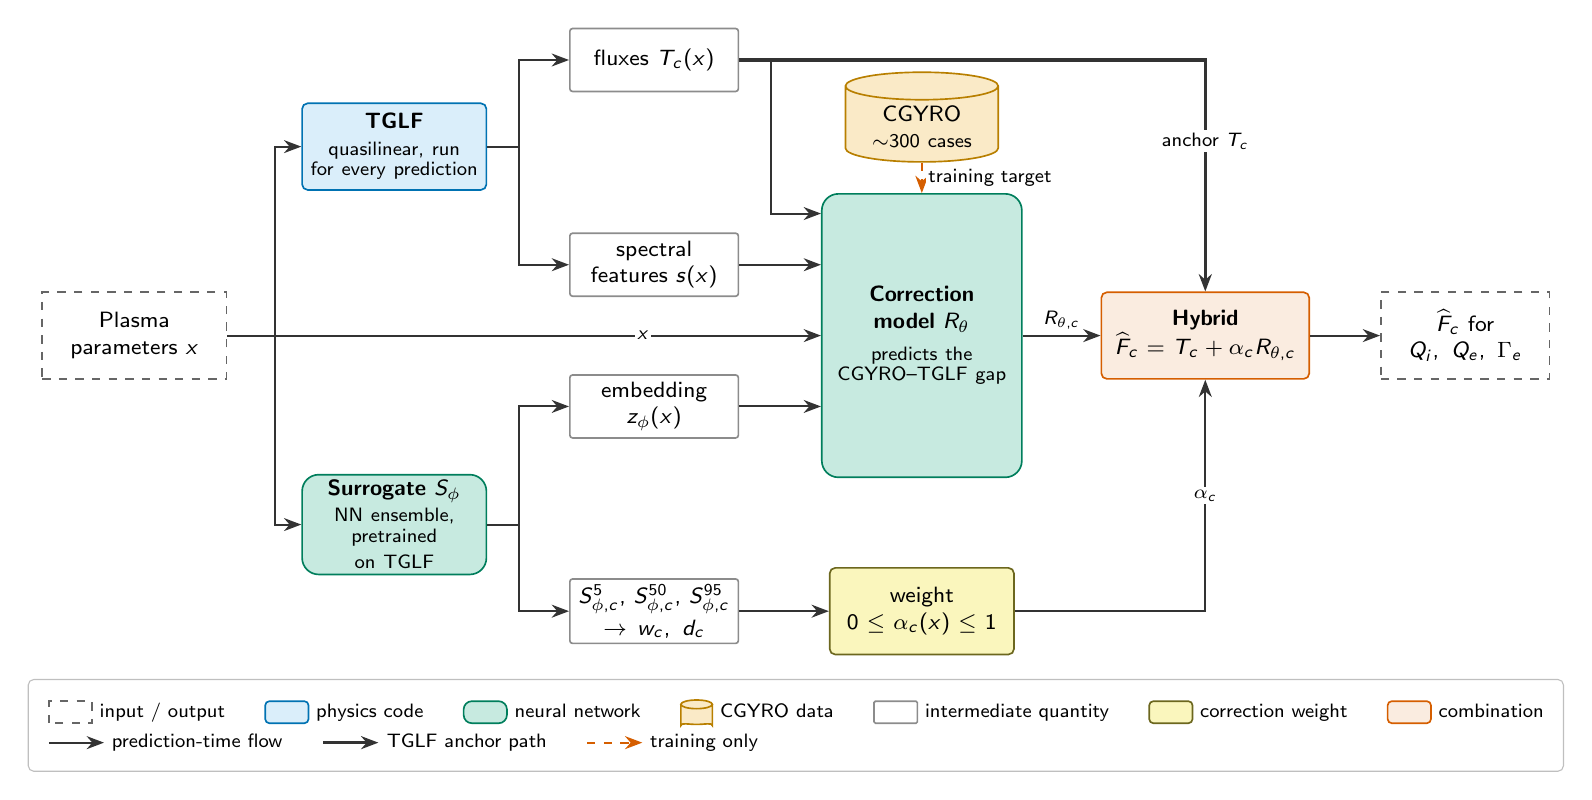
\begin{tikzpicture}

% ---- columns ----
\node[ext] (x) at (0,0) {Plasma\\parameters $x$};

\node[proc]  (tglf) at (3.3, 2.4)  {\textbf{TGLF}\\{\scriptsize quasilinear, run}\\[-2pt]{\scriptsize for every prediction}};
\node[model] (sur)  at (3.3,-2.4)  {\textbf{Surrogate} $S_\phi$\\{\scriptsize NN ensemble,}\\[-2pt]{\scriptsize pretrained on TGLF}};

\node[data] (T)  at (6.6, 3.5) {fluxes $T_c(x)$};
\node[data] (s)  at (6.6, 0.9) {spectral\\features $s(x)$};
\node[data] (z)  at (6.6,-0.9) {embedding $z_\phi(x)$};
\node[data] (wd) at (6.6,-3.5) {$S^{5}_{\phi,c},\,S^{50}_{\phi,c},\,S^{95}_{\phi,c}$\\[1pt]$\to w_c,\ d_c$};

\node[model, minimum height=36mm, text width=24mm] (R) at (10.0,0)
      {\textbf{Correction}\\\textbf{model} $R_\theta$\\[2pt]{\scriptsize predicts the}\\[-2pt]{\scriptsize CGYRO--TGLF gap}};
\node[gate] (a) at (10.0,-3.5) {weight\\$0\le\alpha_c(x)\le 1$};

\node[store] (cg) at (10.0, 2.65) {CGYRO\\{\scriptsize $\sim$300 cases}};

\node[comb] (H) at (13.6,0) {\textbf{Hybrid}\\[1pt]$\widehat F_c = T_c + \alpha_c R_{\theta,c}$};
\node[ext, text width=20mm] (out) at (16.9,0) {$\widehat F_c$ for\\$Q_i,\ Q_e,\ \Gamma_e$};

% ---- x fans out ----
\draw[arr] (x.east) -- ++(6mm,0) |- (tglf.west);
\draw[arr] (x.east) -- ++(6mm,0) |- (sur.west);
\draw[arr] (x.east) -- node[lbl, pos=0.7] {$x$} (R.west);

% ---- TGLF outputs ----
\draw[arr] (tglf.east) -- ++(4mm,0) |- (T.west);
\draw[arr] (tglf.east) -- ++(4mm,0) |- (s.west);

% ---- surrogate outputs ----
\draw[arr] (sur.east) -- ++(4mm,0) |- (z.west);
\draw[arr] (sur.east) -- ++(4mm,0) |- (wd.west);

% ---- into the correction ----
\draw[arr] (T.east) -- ++(4mm,0) |- ([yshift=15.5mm]R.west);
\draw[arr] (s.east) -- ([yshift=0mm]R.west |- s.east);
\draw[arr] (z.east) -- ([yshift=0mm]R.west |- z.east);
\draw[arr] (wd.east) -- (a.west);
\draw[train] (cg.south) -- node[lbl, right=1pt] {training target} (R.north);

% ---- TGLF anchor path to the hybrid ----
\draw[arr, line width=1.1pt] (T.east) -- (H.north |- T.east) -- node[lbl, pos=0.35] {anchor $T_c$} (H.north);
\draw[arr] (R.east) -- node[lbl, above=1pt] {$R_{\theta,c}$} (H.west);
\draw[arr] (a.east) -| node[lbl, pos=0.75] {$\alpha_c$} (H.south);
\draw[arr] (H) -- (out);

% ---- legend ----
\node[anchor=north, font=\scriptsize, align=left, draw=black!25, rounded corners=2pt, inner sep=2.5mm]
     at ($(current bounding box.south)+(0,-3mm)$) {%
  \boxswatch[0pt]{fill=white, draw=black!60, dashed}\ input / output\gap
  \boxswatch{fill=oiSky!22, draw=oiBlue}\ physics code\gap
  \boxswatch[3pt]{fill=oiGreen!22, draw=oiGreen!80!black}\ neural network\gap
  \cylswatch\ CGYRO data\gap
  \boxswatch[0.5pt]{fill=white, draw=black!45}\ intermediate quantity\gap
  \boxswatch{fill=oiYellow!35, draw=oiYellow!45!black}\ correction weight\gap
  \boxswatch{fill=oiVermil!12, draw=oiVermil}\ combination\\[3pt]
  \arrswatch{arr}\ prediction-time flow\gap
  \arrswatch{arr, line width=1.1pt}\ TGLF anchor path\gap
  \arrswatch{train}\ training only};

\end{tikzpicture}
\end{document}
